% Global: reproducible manuscript; local: generated numerical sections read measured artifacts only.
\documentclass[11pt]{article}
\usepackage[margin=1in]{geometry}
\usepackage[T1]{fontenc}
\usepackage{lmodern,amsmath,amssymb,booktabs,graphicx,longtable}
\usepackage[hidelinks]{hyperref}
\usepackage{microtype}
\usepackage{placeins} % Local: keep empirical floats inside Results, before interpretation.
\title{GPhyT With and Without Attention Residuals:\\A Budgeted Paired Architecture Study}
\author{Libor Burian}
\date{October 2026}
\begin{document}
\maketitle
\begin{abstract}
% Global: explicit pre-results status; local: reporting replaces this with measured summaries.
We specify a paired architecture study of Attention Residuals in the General Physics Transformer (GPhyT), reusing the released GPhyT backbone and the Flash Linear Attention reference operator. The planned comparison trains standard and Block Attention Residual variants from scratch at six paired seeds, with three-seed Full and uniform-routing controls. Two selected physics datasets are evaluated at $128\times64$ resolution using fixed autoregressive windows and a final fixed-update checkpoint. The primary endpoint is the equally weighted two-dataset log ratio of 12-step normalized mean squared error. The total project allocation is 24 GPU-hours. At this manuscript revision, implementation checks and prospective power calculations are available, but confirmatory training and test results are pending. No accuracy or stability improvement is established.

All four trained variants nevertheless perform far worse than persistence on convection under the prespecified metric. Radiative forecasts improve in error but produce negative-density cells. The relative architecture result therefore does not establish a physically reliable surrogate or a general advantage of learned routing over fixed averaging.
\end{abstract}
% Global: scientific specification; local: definitions match the versioned implementation.
\section{Context, motivation, and question}
GPhyT uses a shared transformer architecture for forecasting heterogeneous physical fields from a short observed context\cite{gphyt,gphytcode}. Attention Residuals replace fixed residual accumulation with content-dependent aggregation across network depth\cite{attnres,fla}. Their reported language-model results do not establish an advantage for physics forecasts. We test the narrower question: under matched initialization, data schedules, and optimizer-update counts, does Block Attention Residual routing reduce GPhyT's autoregressive prediction error on two selected simulation datasets?

The minimum practically meaningful reduction is prespecified as 5\%. Evidence is conditional on the selected data, resolution, architecture, and compute budget. A confidence interval whose upper improvement bound is below 5\% contradicts that practical hypothesis at the tested scale; an interval spanning the threshold is inconclusive. Failure to reject a zero-effect null is not evidence of equivalence. This distinction follows general recommendations to separate empirical evidence, speculation, and limitations\cite{lones,lipton}.

\section{Background and related implementations}
The Well provides simulations with explicit trajectory splits and physical field metadata\cite{well}. We use its uniform-grid Rayleigh--B\'enard variant and two-dimensional turbulent radiative layer. The uniform-grid correction matters: the original convection data included a nonuniform spatial coordinate, and the maintainers released a separately resampled uniform version\cite{wellrelease}.

We reuse the released GPhyT code at commit \texttt{df1527c}; this is an architecture study trained from scratch, not a reproduction of its broad foundation-model training. For depth aggregation, we vendor the MIT-licensed FLA \texttt{naive\_attnres} implementation at commit \texttt{a400aff6}, preserving source and license\cite{fla}. Fast-AttnRes and Liger provide optimized implementations that introduce Triton-specific execution dependencies\cite{fastattnres,liger}. We also inspected nktkt's standalone implementation\cite{nktkt}. Our source scheduling is specified directly below and tested against raw sublayer outputs, rather than inheriting a third-party transformer integration. The reviewed alternatives, complete revisions, source URLs, and byte hashes are in the public repository\cite{studycode}.

\section{Method}
\begin{figure}[ht]
\centering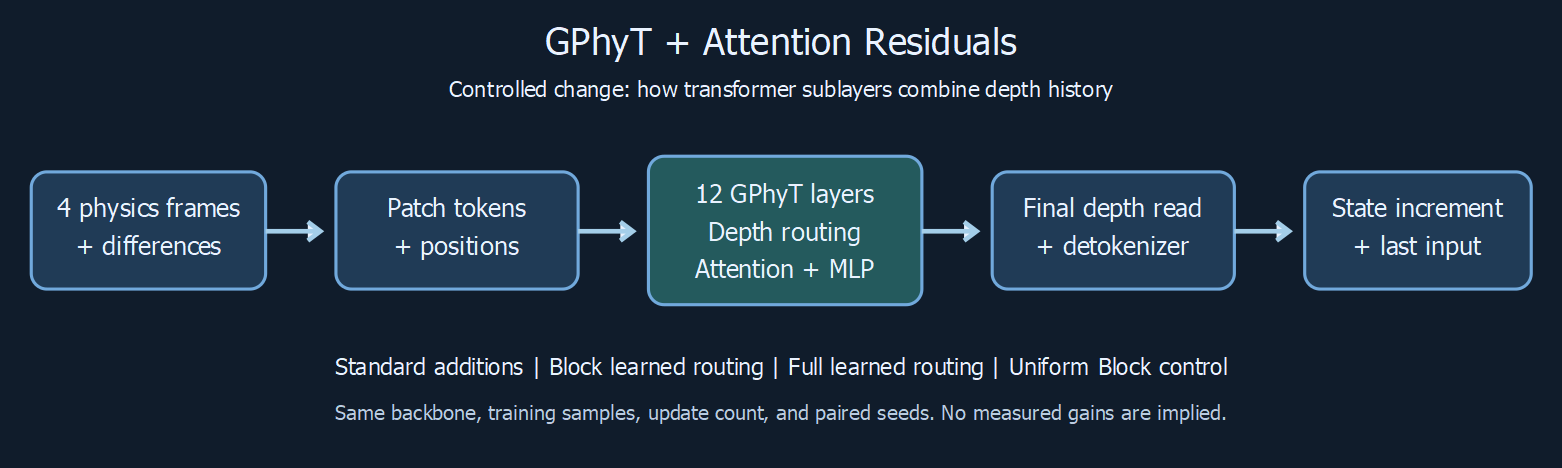
\includegraphics[width=\linewidth]{../reports/figures/architecture.png}
\caption{Controlled architectural change. All variants reuse the same upstream transformations and outer next-state update; only depth composition changes.}
\end{figure}
\subsection{Controlled architecture change}
The backbone has twelve transformer layers, hidden width 192, MLP width 768, three attention heads, absolute positional embeddings, and $1\times16\times16$ spatiotemporal patches. Four context frames at $128\times64$ give 128 tokens. We preserve the upstream tokenizer, positional embeddings, attention, MLPs, finite-difference features, and detokenizer. The upstream forward computes an increment for each context position, adds the original input, and returns the final position. Although the upstream class stores an integrator, this forward does not execute Runge--Kutta integration or use the \texttt{step\_size} argument\cite{gphytcode}.

Write the tokenizer-plus-position output as $e$, and raw attention or MLP output at sublayer $\ell$ as $v_\ell=F_\ell(h_\ell)$. Each $F_\ell$ retains its original normalization. Given the causally available source bank $S_\ell$, our depth read is
\begin{align}
 k_{\ell i} &= \gamma_\ell\odot s_i\left(d^{-1}\sum_{j=1}^{d}s_{ij}^2+10^{-6}\right)^{-1/2},\\
 a_{\ell i} &= \frac{\exp(q_\ell^\top k_{\ell i})}{\sum_{s_r\in S_\ell}\exp(q_\ell^\top k_{\ell r})},
 &h_\ell &=\sum_{s_i\in S_\ell}a_{\ell i}s_i .
\end{align}
These operations apply independently at each token. The query $q_\ell$ starts at zero and the key scale $\gamma_\ell$ at one\cite{attnres,fla}. Mathematically, the initial read is an arithmetic mean, not a sum. Values are the unnormalized sources; only keys are RMS-normalized. There is no additional inverse-square-root attention scale in this operator.

Full routing stores $S_\ell=\{e,v_1,\ldots,v_{\ell-1}\}$. Block routing stores the embedding, completed sums of four consecutive sublayer outputs, and a nonempty partial sum for the current block. A completed sum appears exactly once: its partial slot is cleared at the boundary. Thus the 24 writers form six blocks. A separate final depth read includes all completed outputs before detokenization. The source bank resets for every forward call. Uniform Block uses exactly these sources with fixed equal weights and no learned routing parameters. Standard residuals call the unchanged upstream block forward. With five canonical channels, execution checks count 7,919,045 backbone parameters; learned routing adds $25\times2\times192=9,600$ parameters. This count is specific to our input/output configuration, rather than the parameter count of a differently configured published model.

\subsection{Data and normalization}
The selected datasets originate from Dedalus convection simulations and Athena++ radiative mixing-layer simulations, respectively; we credit their original numerical and physical work\cite{dedalus,fielding} in addition to The Well distribution\cite{well}.
The convection selection fixes Prandtl number 1 and Rayleigh numbers $10^6$, $10^8$, and $10^{10}$. The radiative selection includes all nine cooling settings. Official train, validation, and test trajectory membership is preserved. Source files, coordinates, parameter identities, SHA-256 hashes, and trajectory hashes are recorded before training. Exact full-trajectory duplication across splits causes preparation to fail. Shared initial-state hashes are disclosed separately because identical starting fields need not imply identical trajectories.

Each field is area-downsampled on CPU to $128\times64$ without transposing or reversing stored spatial axes. The canonical channel vector is pressure, density, buoyancy, velocity $x$, and velocity $y$. Buoyancy is not relabeled as temperature. Absent fields are zero, are masked out of optimization and error metrics, and remain zero in autoregressive feedback. Per-dataset, per-active-field means and standard deviations use all selected training trajectories only. Validation/test targets do not enter normalization.

The convection split contains 120 training, 15 validation, and 15 test trajectories; the corresponding radiative counts are 72, nine, and nine. Original grids are $512\times128$ and $128\times384$, with 200 and 101 frames per trajectory. No exact full-trajectory hash crosses splits. There are 33 distinct cross-split first-frame hash groups (25 convection, eight radiative), all spanning different parameter settings; every held-out trajectory shares an initial state with training under another setting. No first-four-frame prepared context is exactly duplicated across splits. This context check is not an exhaustive search over all possible windows. The public manifest and separate audit record all member identities\cite{studycode}.

Training samples are drawn uniformly by dataset, then parameter setting, trajectory, stride in $\{1,\ldots,8\}$, and a valid start index. Four strided context frames predict the fifth. The model receives no explicit parameter label or stride value. Validation monitoring uses a separate fixed sampling generator and cannot advance the training sequence. Evaluation uses stride one and three prespecified start fractions, $0$, $1/2$, and $1$, of the valid origin range for four context plus 24 forecast frames.

\subsection{Optimization and compute allocation}
Under BF16 autocast, the upstream learned FP32 positional embedding promotes the residual stream to FP32. We promote raw sublayer outputs to that same stream dtype before depth-block summation, preserving the standard path's accumulation precision. The attention and MLP matrix operations retain BF16 autocast; this is mixed precision rather than a fully BF16 residual accumulator. Routing also executes inside autocast: FLA's explicit FP32 casts do not prevent its eligible contractions from being autocast\cite{pytorchamp}. The original protocol incorrectly described routing as entirely FP32. This discrepancy was disclosed during training; the frozen training computation was not changed. CPU BF16 regression checks reproduce the distinction; they are not measurements of CUDA rounding error.
Standard and Block variants share seeds 0--5; Full and Uniform Block use seeds 0--2. Backbone initialization is identical within each seed across variants. Data RNGs are independent of model construction and timing, producing paired examples. Standard/Block execution order is randomized within each seed using a fixed scheduling RNG; all primary pairs precede exploratory controls.

Real-data profiling selected microbatch four and froze 3,175 optimizer updates per run, with effective batch sixteen (50,800 sampled examples per run). The fixed cost rule projects 14.400 training hours across all eighteen runs. On the RTX 5070 Laptop GPU with PyTorch 2.14.1+cu130, median update times were 0.7760/0.7913/0.8914/0.8471 seconds for Standard/Block/Full/Uniform, respectively. Each median uses sixteen updates after two warm-ups; these short measurements set the horizon rather than establish a throughput ranking. The profile consumed 71.144 seconds; the previous execution checks consumed 2.920 seconds. The source-linked frozen artifact retains all timings, overhead measurements, hardware identity, sample order, and the portable data fingerprint\cite{studycode}.

All variants use AdamW with learning rate $10^{-4}$, weight decay $10^{-4}$, $(\beta_1,\beta_2)=(0.9,0.999)$, and $\epsilon=10^{-8}$. We clip the accumulated gradient norm to 1, use effective batch size 16, BF16 autocast with FP32 loss reduction, 5\% linear warmup, and cosine decay to $10^{-6}$. A common microbatch is selected from 4, 2, and 1 by memory feasibility. Dropout and stochastic depth remain zero.

The 24 GPU-hour cap allocates 2 hours to profiling/validation, 18 to training, 2 to evaluation, and 2 to contingencies. An exclusive persistent ledger includes failed GPU attempts and wall time spent on IO inside GPU phases. CPU data preparation is outside the GPU allocation. Profiling measures actual optimizer updates for all variants, validation, and checkpoint serialization. A single update count is chosen using measured 90th-percentile update costs, amortized overhead, run multiplicities, and a prespecified 20\% safety margin. This count is published before confirmatory training. The final fixed-update checkpoint defines the endpoint; validation scores never select a better checkpoint.

\subsection{Metrics and statistical analysis}
For standardized target $y$ and prediction $\hat y$, field $c$, and forecast step $t$,
\begin{equation}
 m_{tc}=\frac{\langle(\hat y_{tc}-y_{tc})^2\rangle_{x,y}}{\langle y_{tc}^2\rangle_{x,y}+10^{-6}}.
\end{equation}
For horizon $H$, errors average equally over active fields and steps $1,\ldots,H$, then predetermined windows within a trajectory, then trajectories within each dataset. The target second moment is computed in training-standardized coordinates; this definition is not a claim to reproduce every normalization convention used in The Well benchmarks.

Let $E_{s,d}^{B}$ and $E_{s,d}^{S}$ denote Block and Standard 12-step dataset errors for seed $s$. The independent paired effect is
\begin{equation}
D_s=\tfrac12\sum_{d=1}^{2}\log(E_{s,d}^{B}/E_{s,d}^{S}),\qquad I=1-\exp(\overline D).
\end{equation}
We report all six paired effects, a Student-$t$ interval for $\overline D$ transformed to $I$, and an exact two-sided test enumerating all $2^6$ sign flips. The interval assumes approximately normal independent seed effects; the randomization test requires within-pair exchangeability under its null. Frames and windows are correlated observations, not independent replicates. Inference is conditional on the fixed test trajectories. With six pairs, the minimum two-sided exact p-value is $2/64=0.03125$. Undefined/divergent trajectory errors propagate to dataset estimates; incomplete primary pairs produce an undefined primary analysis rather than a reduced successful-only sample.

Prospective power sensitivity uses assumed Gaussian paired log ratios with standard deviations $0.02$, $0.05$, $0.10$, and $0.20$, and improvements of 5\%, 10\%, and 20\%. It includes noncentral-$t$ power and 100,000 independent simulated exact tests per condition, with simulation RNG seed 20261025. These are assumptions, not estimated post-hoc power.

\subsection{Secondary outcomes and interventions}
Secondary outcomes include one-step and 24-step NMSE, persistence, per-dataset errors, throughput, peak memory, gradient norms, and depth-routing weights. Physical diagnostics include radiative negative-pressure/density fractions and convection velocity-divergence residuals compared with coarsened ground truth using stored physical grid spacing. They do not assert exact conservation or solver equivalence.

On the first four test trajectories per dataset in manifest order, trained Block models are re-evaluated with uniform routing weights and with a fixed-RNG depth permutation of learned weights. These are within-model interventions, not separately retrained models or proof that a mechanism mediates all architecture differences. Their sources and parameters are unchanged; only routing weights are intervened upon. Before test evaluation, an implementation audit replaced the intervention's pointwise FP32 reduction with the same flattened contraction used by ordinary FLA routing. This prevents an additional arithmetic change when weights are held fixed. Exploratory comparisons are reported descriptively without converting secondary tests into a replacement primary endpoint.

\section{Results}
\subsection{Radiative-flow highlight: lowest mean error among tested baselines}
On this study's radiative-flow full test set, GPhyT + Block Attention Residuals has the lowest mean 12-step NMSE among all nine tested trained, initialized, and persistence models: 0.28917. That is 26.38\% lower than GPhyT without Attention Residuals (0.39277) and 30.99\% lower than persistence (0.41901).
This is a descriptive mean ranking, emphasized after results, not a win in every seed. Standard/Block use six seeds and Full/Uniform three; initialized controls are post-hoc. The preregistered two-dataset test remains separate and does not establish significance against every comparator.
\subsection{Unchanged preregistered two-dataset comparison}
At this report revision, 18 of 18 planned training runs are complete. Block Attention Residuals reduce the primary error endpoint by 24.52\% relative to GPhyT without Attention Residuals, with 95\% confidence interval [11.56, 35.58]\% and exact paired p-value 0.03125. These estimates condition on the selected datasets and fixed evaluation windows.
The interval supports the prespecified minimum 5\% improvement.
\begin{figure}[ht]\centering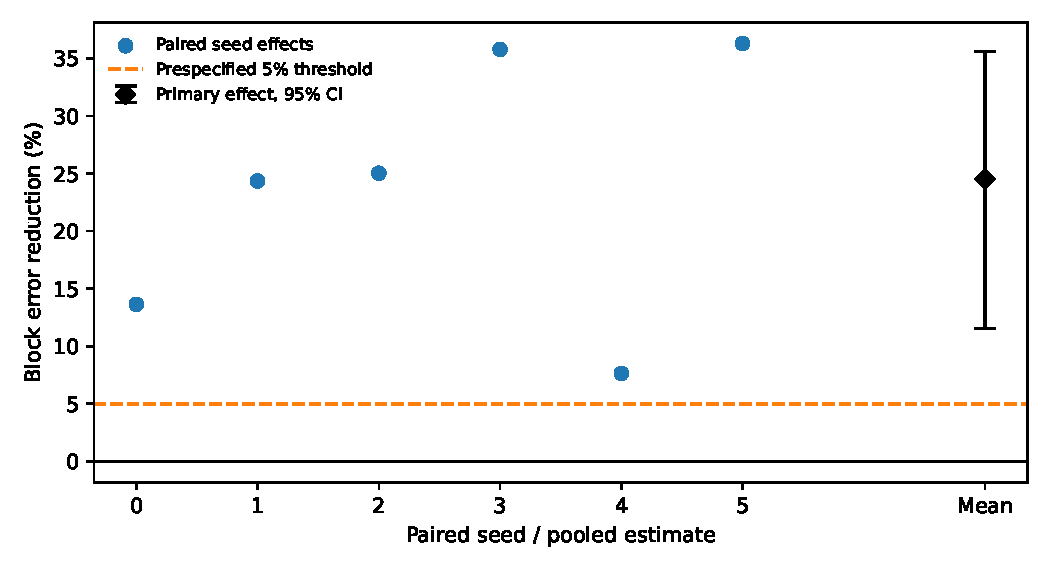
\includegraphics[width=.95\linewidth]{../reports/figures/paired_effects.pdf}\caption{All six paired seed effects and the primary transformed t confidence interval. The dashed line is the prespecified practical threshold.}\end{figure}
\begin{table}[ht]\centering\small
\begin{tabular}{lll}
\toprule
Model & Convection & Radiative \\
\midrule
GPhyT without Attention Residuals & 39284.2 & 0.392769 \\
GPhyT + Block AttnRes & 30006 & 0.289174 \\
\bottomrule
\end{tabular}
\caption{Primary baseline comparison: arithmetic mean twelve-step NMSE across the same six seeds (lower is better). Both models train from scratch with identical shared-parameter initialization, paired sampled examples, optimizer schedule, update count, and effective batch size. Compute cost differs by architecture. The preregistered two-dataset relative reduction uses paired dataset log-error ratios, not the ratio of these arithmetic means.}\end{table}
\begin{table}[ht]\centering\small
\begin{tabular}{llllll}
\toprule
Dataset & Model & Finite/planned & 1 step & 12 step & 24 step \\
\midrule
Convection & No AttnRes & 6/6 & 334.8 & 3.928e+04 & 4.561e+04 \\
Convection & Block & 6/6 & 181.8 & 3.001e+04 & 4.076e+04 \\
Convection & Full & 3/3 & 93.01 & 1.84e+04 & 3.126e+04 \\
Convection & Uniform & 3/3 & 200.6 & 2.499e+04 & 2.898e+04 \\
Convection & Persistence & 1/1 & 0.04142 & 0.2174 & 0.3296 \\
Radiative & No AttnRes & 6/6 & 0.1422 & 0.3928 & 0.7028 \\
Radiative & Block & 6/6 & 0.1332 & 0.2892 & 0.427 \\
Radiative & Full & 3/3 & 0.1381 & 0.3174 & 0.4357 \\
Radiative & Uniform & 3/3 & 0.1446 & 0.3473 & 0.5948 \\
Radiative & Persistence & 1/1 & 0.1529 & 0.419 & 0.5403 \\
\bottomrule
\end{tabular}
\caption{Arithmetic mean seed NMSE for each fixed horizon. No AttnRes denotes GPhyT without Attention Residuals. A horizon averages all forecast steps up to that horizon. Architecture means require every planned seed to have a finite endpoint. Finite/planned counts refer to twelve steps; persistence is a deterministic baseline, not a one-seed uncertainty estimate. Complete descriptive seed SDs and t intervals are in accuracy\_summary.csv.}\end{table}
\begin{figure}[ht]\centering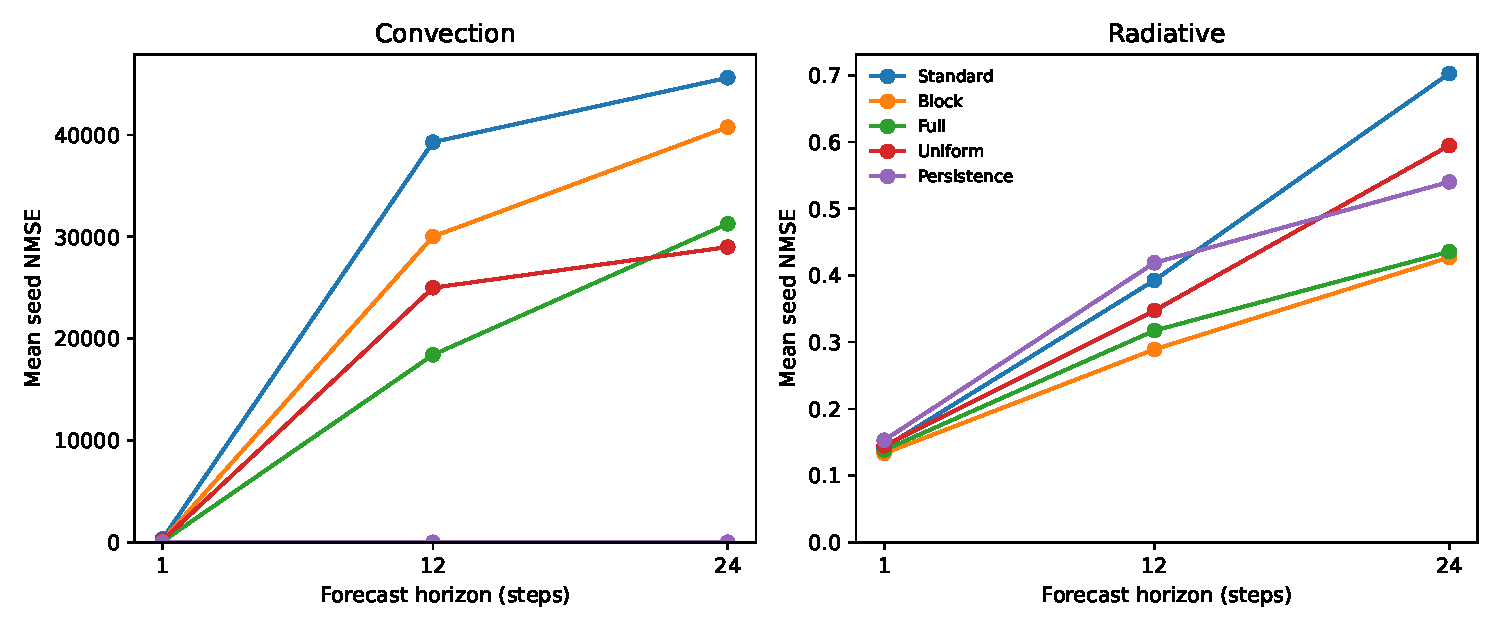
\includegraphics[width=\linewidth]{../reports/figures/forecast_errors.pdf}\caption{Fixed-horizon trajectory-averaged errors for both datasets. Missing values remain missing.}\end{figure}
\begin{table}[ht]\centering\scriptsize
\begin{tabular}{lrrrr}
\toprule
Run & Updates & Wall seconds & Examples/s & Peak MiB \\
\midrule
block\_seed0 & 3175 & 2473.97 & 20.68 & 365.88 \\
block\_seed1 & 3175 & 2011.53 & 25.65 & 365.88 \\
block\_seed2 & 3175 & 2639.13 & 19.30 & 365.88 \\
block\_seed3 & 3175 & 2547.29 & 20.36 & 365.88 \\
block\_seed4 & 3175 & 2522.62 & 20.63 & 365.88 \\
block\_seed5 & 3175 & 2568.18 & 20.49 & 365.88 \\
full\_seed0 & 3175 & 2966.65 & 18.11 & 546.00 \\
full\_seed1 & 3175 & 2829.46 & 18.36 & 546.00 \\
full\_seed2 & 3175 & 2473.04 & 20.80 & 546.00 \\
standard\_seed0 & 3175 & 2191.09 & 26.75 & 278.46 \\
standard\_seed1 & 3175 & 1282.01 & 41.12 & 278.46 \\
standard\_seed2 & 3175 & 1510.54 & 33.42 & 278.46 \\
standard\_seed3 & 3175 & 1459.29 & 35.46 & 278.46 \\
standard\_seed4 & 3175 & 1488.47 & 35.03 & 278.46 \\
standard\_seed5 & 3175 & 1490.51 & 34.76 & 278.46 \\
uniform\_block\_seed0 & 3175 & 2655.30 & 20.01 & 345.86 \\
uniform\_block\_seed1 & 3175 & 2470.89 & 21.12 & 345.86 \\
uniform\_block\_seed2 & 3175 & 2238.16 & 23.09 & 345.86 \\
\bottomrule
\end{tabular}
\caption{Per-run cost, including failed or incomplete runs. Examples/s uses the median synchronized update time; wall seconds also include validation and checkpointing. Peak memory is PyTorch allocated device memory.}\end{table}
\begin{table}[ht]\centering\small
\begin{tabular}{lll}
\toprule
Model / routing control & Convection & Radiative \\
\midrule
Block: original & 17550.8 & 0.297138 \\
Block: uniform intervention & 42767.8 & 2.16975 \\
Block: shuffled (random) intervention & 40924 & 2.81369 \\
\bottomrule
\end{tabular}
\caption{Absolute twelve-step NMSE on the matched diagnostic subset: first four test trajectories per dataset, averaged across all six trained Block seeds. The original reference is evaluated on exactly this subset, not the full test population in the baseline tables. Uniform replaces routing weights by equal weights; shuffled is the random control, permuting learned depth-weight assignments with RNG seed 20261025. Neither intervention is retrained. Seed counts, SDs, and descriptive intervals are in intervention\_accuracy\_summary.csv.}\end{table}
\begin{table}[ht]\centering\small
\begin{tabular}{lllrr}
\toprule
Dataset & Routing & Finite/planned & Mean error ratio & Seed SD \\
\midrule
Convection & shuffle & 6/6 & 2.63 & 1.245 \\
Convection & uniform & 6/6 & 2.565 & 0.7757 \\
Radiative & shuffle & 6/6 & 9.524 & 5.603 \\
Radiative & uniform & 6/6 & 7.49 & 6.105 \\
\bottomrule
\end{tabular}
\caption{Within-model twelve-step routing interventions on the same first four test trajectories per dataset. Values are intervened/original NMSE ratios, averaged over trained Block seeds. These are exploratory diagnostics, not independently trained controls or evidence of a unique mechanism.}\end{table}
\begin{table}[ht]\centering\scriptsize
\begin{tabular}{llrrr}
\toprule
Dataset & Diagnostic & Standard & Block & Persistence \\
\midrule
Convection & Divergence error RMS & 4.13 & 2.82 & 0.228 \\
Convection & Predicted divergence RMS & 4.13 & 2.81 & 0.165 \\
Convection & Target divergence RMS & 0.175 & 0.175 & 0.175 \\
Radiative & Negative density fraction & 0.26 & 0.273 & 0 \\
Radiative & Negative pressure fraction & 0 & 0 & 0 \\
\bottomrule
\end{tabular}
\caption{Secondary physical diagnostics averaged over all 24 forecast steps, then windows, trajectories, and complete planned seed sets. Divergence uses the stored physical coordinates and coarsened target; positivity rates are fractions. These diagnostics do not establish exact conservation. All architectures and interventions are retained in physical\_diagnostics.csv.}\end{table}
Across the available ordinary evaluations, 0/1368 forecast windows have undefined twelve-step error, and 0/1368 have undefined twenty-four-step error. These descriptive counts include persistence and repeated model evaluations; they are not independent replicates or an inferential sample size. Per-run counts are preserved in rollout\_stability.csv.
\begin{figure}[ht]\centering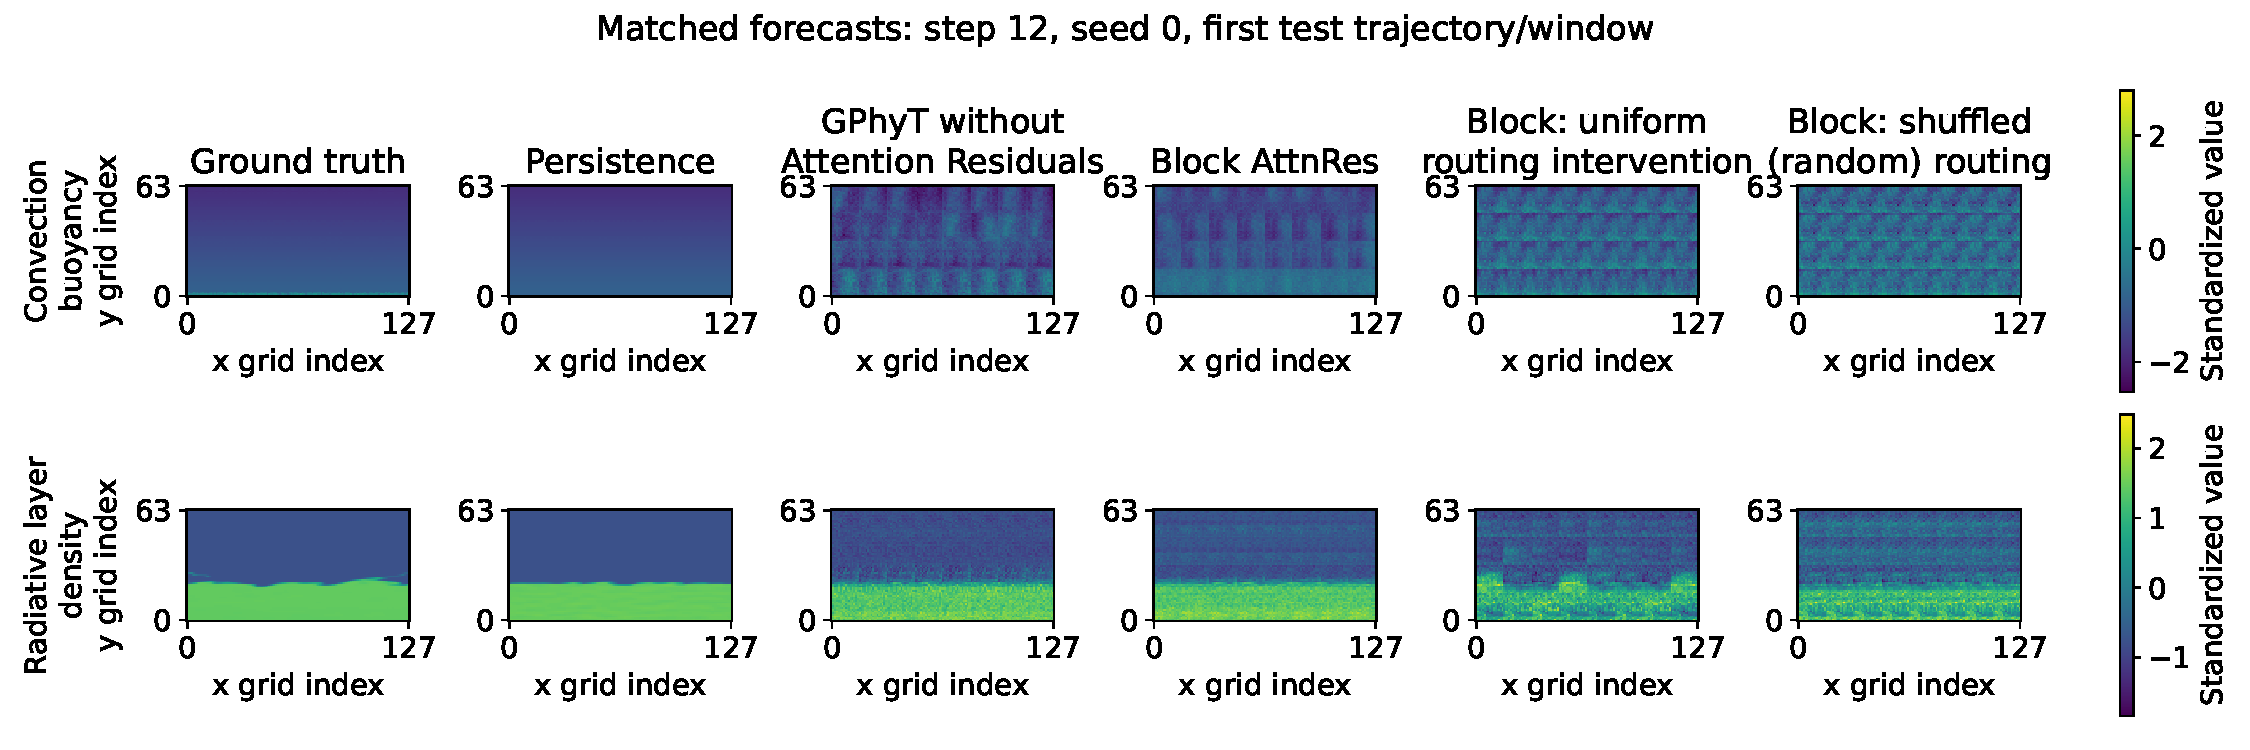
\includegraphics[width=\linewidth]{../reports/figures/control_comparison.pdf}\caption{Baselines, new method, and controls on the same first test trajectory/window at step twelve: persistence, GPhyT without Attention Residuals, ordinary Block, and Block with uniform or randomly shuffled depth weights. Interventions use the same trained seed-zero Block checkpoint without retraining; shuffling preserves learned weight magnitudes but permutes source assignments with fixed RNG seed 20261025. Persistence repeats the last observed context frame. Rows show convection buoyancy and radiative density with one shared, unclipped color scale per row in training-standardized units. This post-result presentation reuses fixed cases and saved intervention forecasts; it introduces no new endpoint or GPU inference.}\end{figure}
\begin{figure}[ht]\centering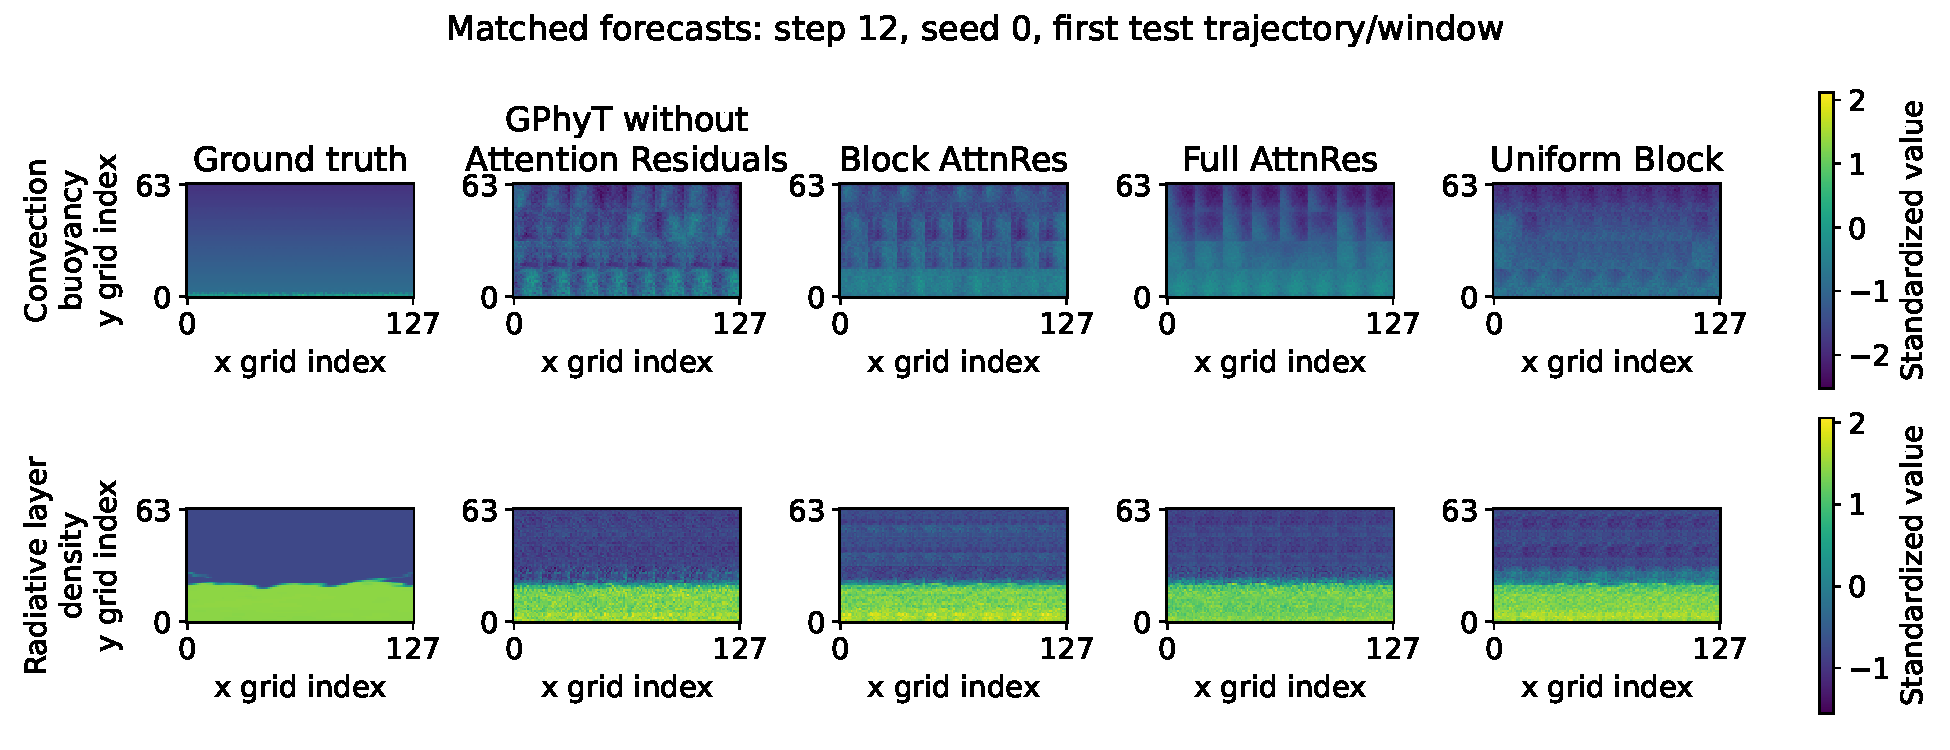
\includegraphics[width=\linewidth]{../reports/figures/field_comparison.pdf}\caption{Ground truth and all four trained architectures on identical held-out cases: seed zero, first test trajectory and first fixed window, forecast step twelve. Each row uses one common color range spanning truth and all predictions, without clipping, in training-standardized units; magenta would mark nonfinite values. Convection shows buoyancy (not temperature); radiative flow shows density. These illustrative fields do not replace the full paired evaluation. The all-model layout was added after results at the user's request, reusing the already fixed preview cases.}\end{figure}
\begin{figure}[ht]\centering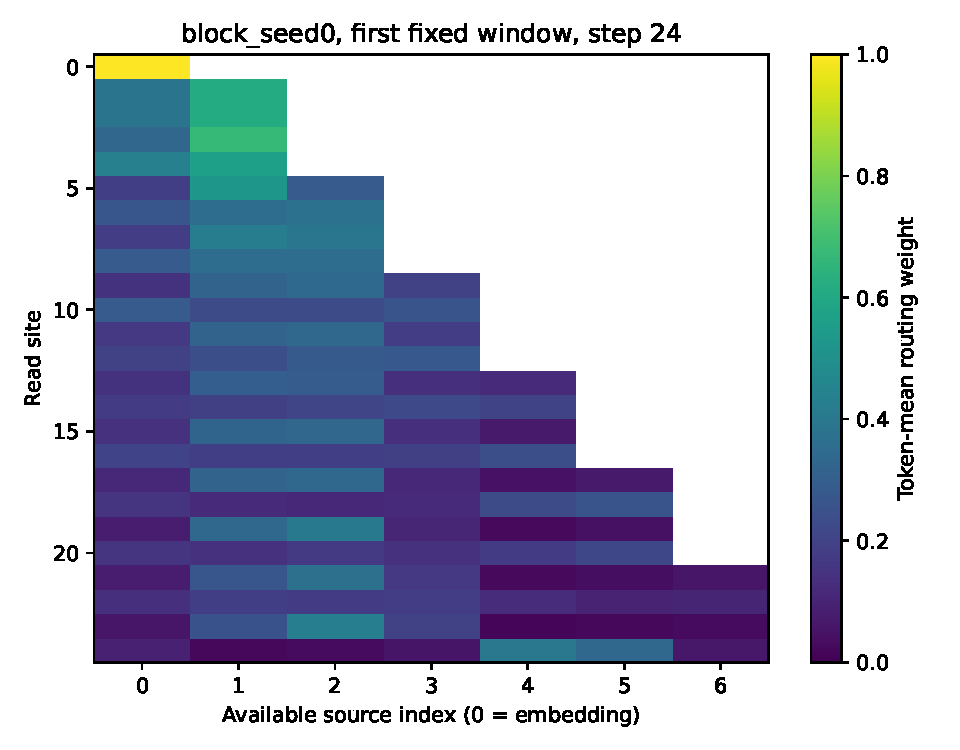
\includegraphics[width=.72\linewidth]{../reports/figures/routing_block_seed0.pdf}\caption{Routing in the prespecified seed-zero, first-trajectory, first-window case. White cells represent unavailable or undefined weights; a heatmap alone does not establish causal importance.}\end{figure}
\begin{figure}[ht]\centering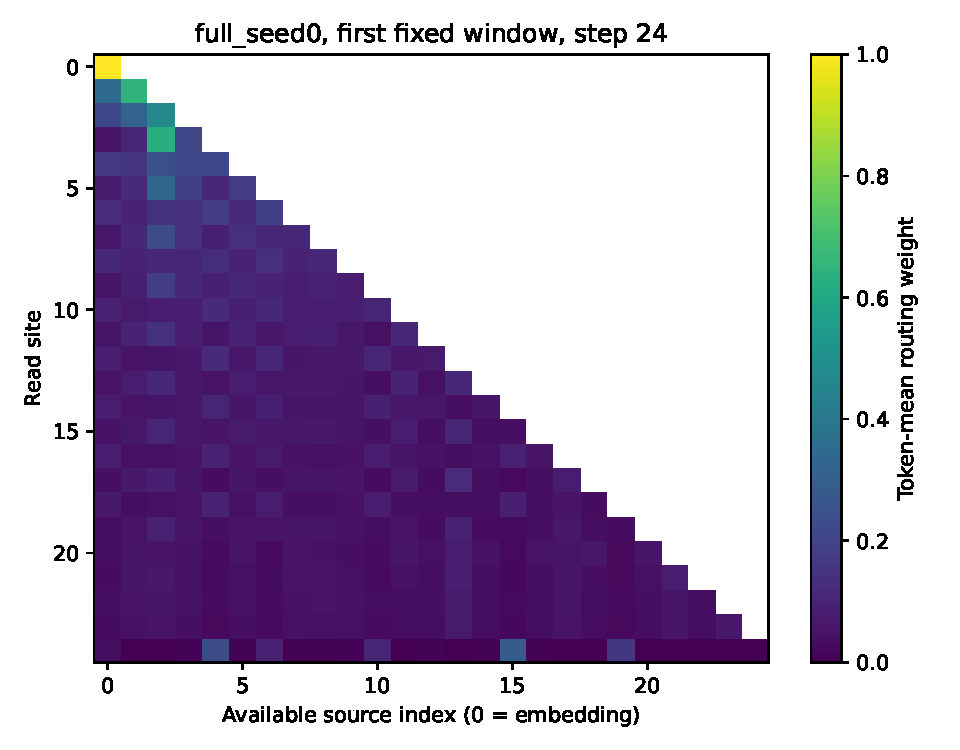
\includegraphics[width=.72\linewidth]{../reports/figures/routing_full_seed0.pdf}\caption{Routing in the prespecified seed-zero, first-trajectory, first-window case. White cells represent unavailable or undefined weights; a heatmap alone does not establish causal importance.}\end{figure}
\begin{figure}[ht]\centering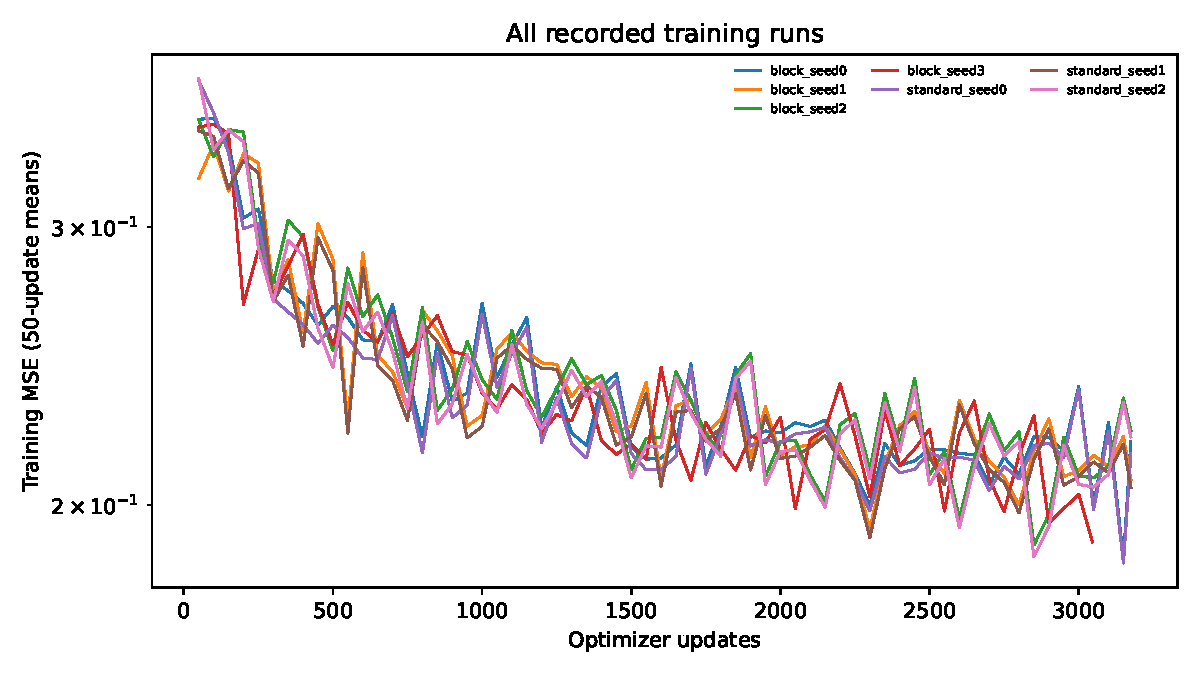
\includegraphics[width=\linewidth]{../reports/figures/learning_curves.pdf}\caption{All recorded runs with fixed fifty-update bins. Full update records accompany the checkpoints. Supervised MSE is a training objective, not a reinforcement-learning reward.}\end{figure}
\begin{figure}[ht]
\centering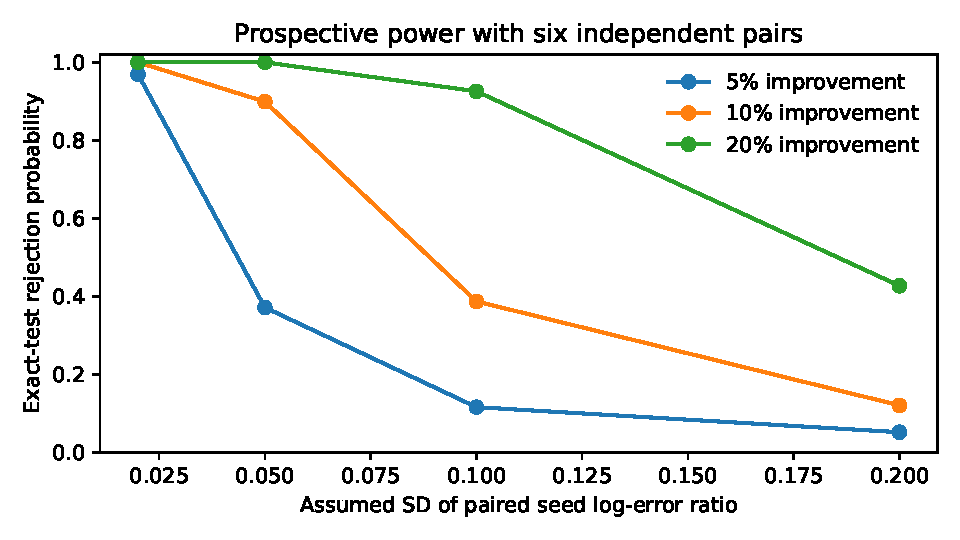
\includegraphics[width=.8\linewidth]{../reports/figures/power_sensitivity.pdf}
\caption{Prospective power under explicitly assumed independent Gaussian seed effects. This is a sensitivity calculation, not observed prediction accuracy.}\end{figure}
For a 5\% improvement, exact-test simulated power is 0.37124 at assumed log-ratio standard deviation 0.05 and 0.11563 at 0.10 (100,000 draws per condition). All sensitivity assumptions and Monte Carlo errors are published.
\clearpage
\subsection{Post-hoc initialization-only baselines}
The additional user-requested zero-update evaluation completed 18/18 planned controls. These controls were specified after observing the trained-model results and do not alter the original confirmatory comparison. The models were reconstructed with the original constructor, configuration, and seeds, without loading trained weights or applying optimizer updates. Parameter and buffer hashes were checked before and after inference.
\begin{table}[ht]\centering\scriptsize
\begin{tabular}{lllll}
\toprule
Dataset & Model & Finite/planned & Initialized & Trained \\
\midrule
Convection & GPhyT without AttnRes & 6/6 & 350742 & 39284.2 \\
Convection & Block AttnRes & 6/6 & 8173.5 & 30006 \\
Convection & Full AttnRes & 3/3 & 1332 & 18397.8 \\
Convection & Uniform Block & 3/3 & 7780.76 & 24987 \\
Radiative & GPhyT without AttnRes & 6/6 & 7.02088 & 0.392769 \\
Radiative & Block AttnRes & 6/6 & 0.572704 & 0.289174 \\
Radiative & Full AttnRes & 3/3 & 0.413095 & 0.317353 \\
Radiative & Uniform Block & 3/3 & 0.524838 & 0.347345 \\
\bottomrule
\end{tabular}
\caption{Twelve-step NMSE for initialized models (zero updates) and their trained counterparts (3,175 updates), on the same complete test population. Standard/Block use seeds 0--5; Full/Uniform use seeds 0--2. Finite/planned counts refer to initialized endpoints; incomplete or divergent seed sets remain undefined. These are descriptive post-hoc controls, not additional confirmatory tests. All horizons and seed uncertainty are in reports/untrained/comparison.csv.}\end{table}
\begin{figure}[ht]\centering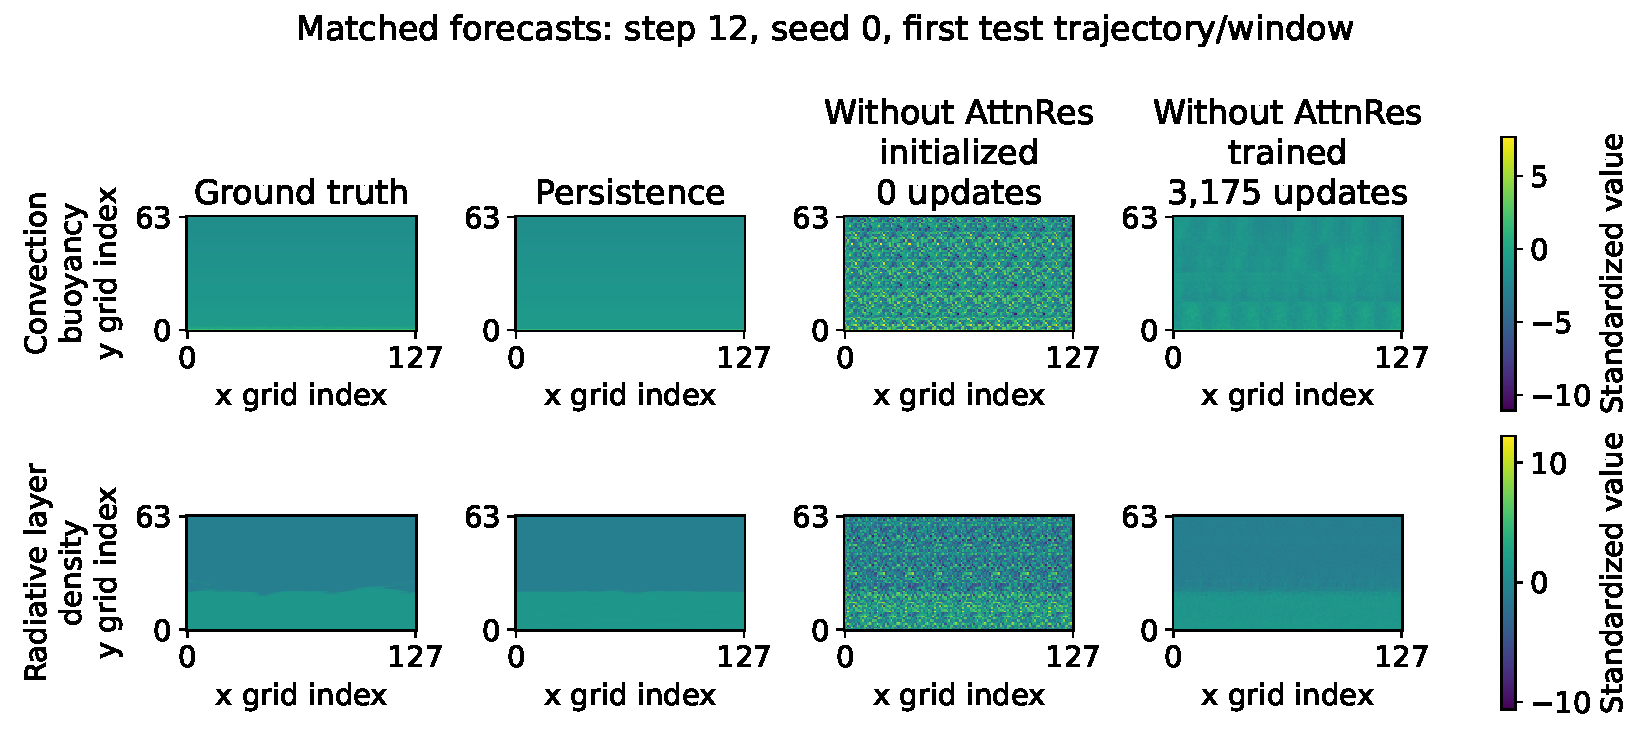
\includegraphics[width=\linewidth]{../reports/figures/initialization_standard.pdf}\caption{Initialized versus trained GPhyT without AttnRes: ground truth, persistence, zero-update model, and final trained checkpoint. Both rows use the same seed-zero first test trajectory/window at forecast step twelve, with one common unclipped color range per row. Top: convection buoyancy; bottom: radiative density. Magenta denotes nonfinite values. These fixed illustrative cases do not replace evaluation over all trajectories and seeds.}\end{figure}
\begin{figure}[ht]\centering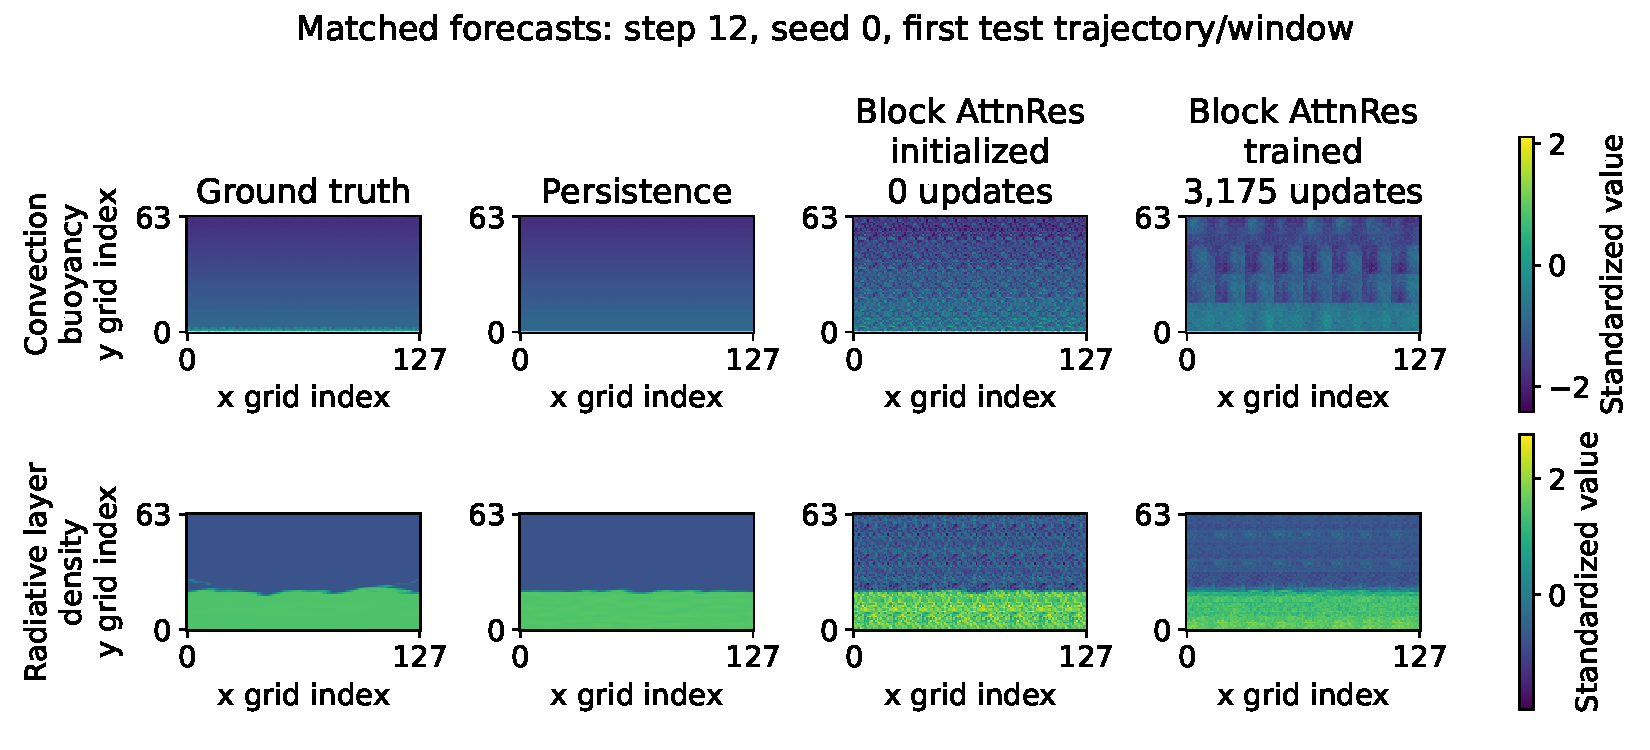
\includegraphics[width=\linewidth]{../reports/figures/initialization_block.pdf}\caption{Initialized versus trained Block AttnRes: ground truth, persistence, zero-update model, and final trained checkpoint. Both rows use the same seed-zero first test trajectory/window at forecast step twelve, with one common unclipped color range per row. Top: convection buoyancy; bottom: radiative density. Magenta denotes nonfinite values. These fixed illustrative cases do not replace evaluation over all trajectories and seeds.}\end{figure}
\begin{figure}[ht]\centering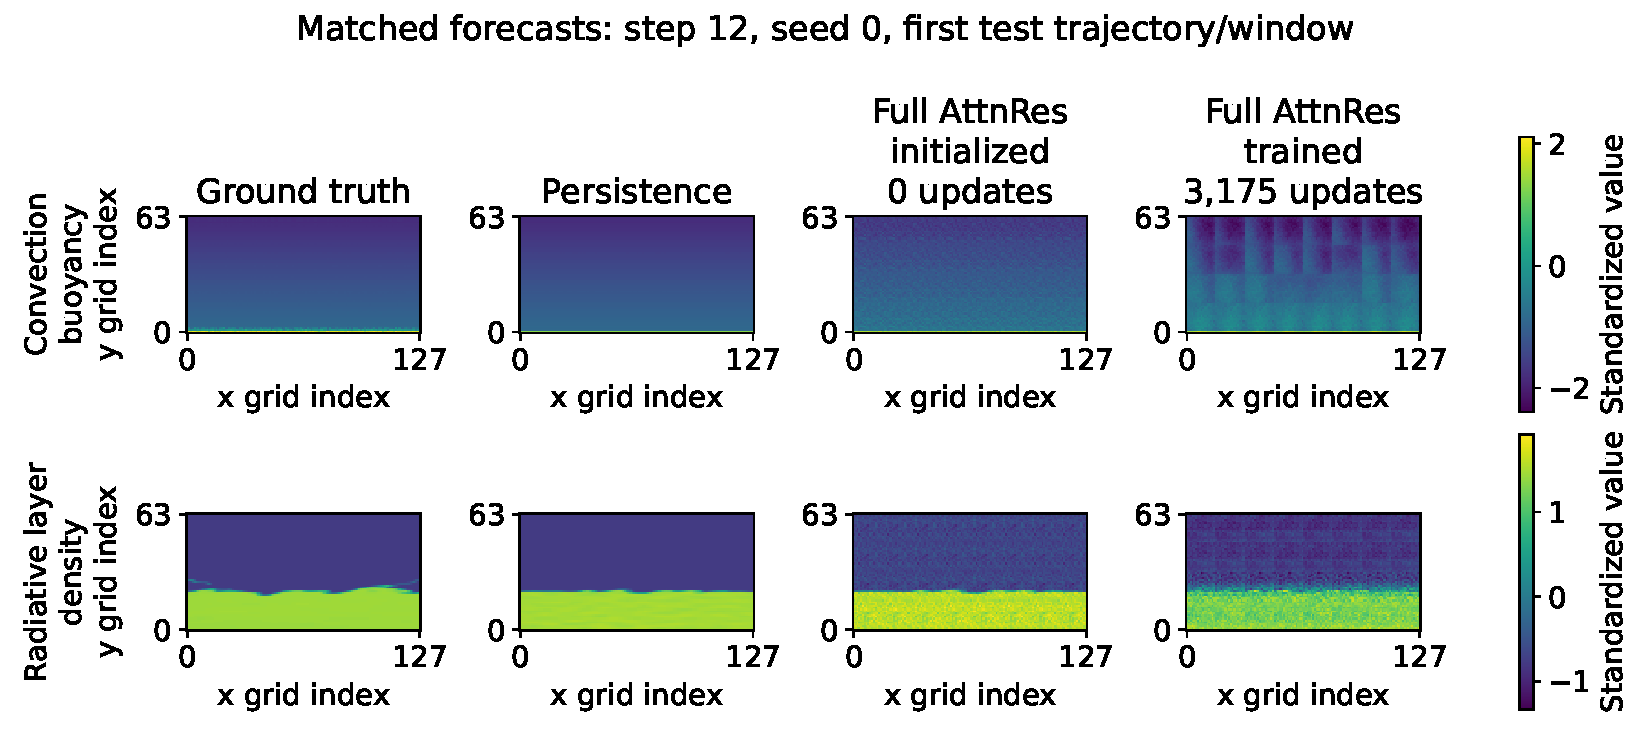
\includegraphics[width=\linewidth]{../reports/figures/initialization_full.pdf}\caption{Initialized versus trained Full AttnRes: ground truth, persistence, zero-update model, and final trained checkpoint. Both rows use the same seed-zero first test trajectory/window at forecast step twelve, with one common unclipped color range per row. Top: convection buoyancy; bottom: radiative density. Magenta denotes nonfinite values. These fixed illustrative cases do not replace evaluation over all trajectories and seeds.}\end{figure}
\begin{figure}[ht]\centering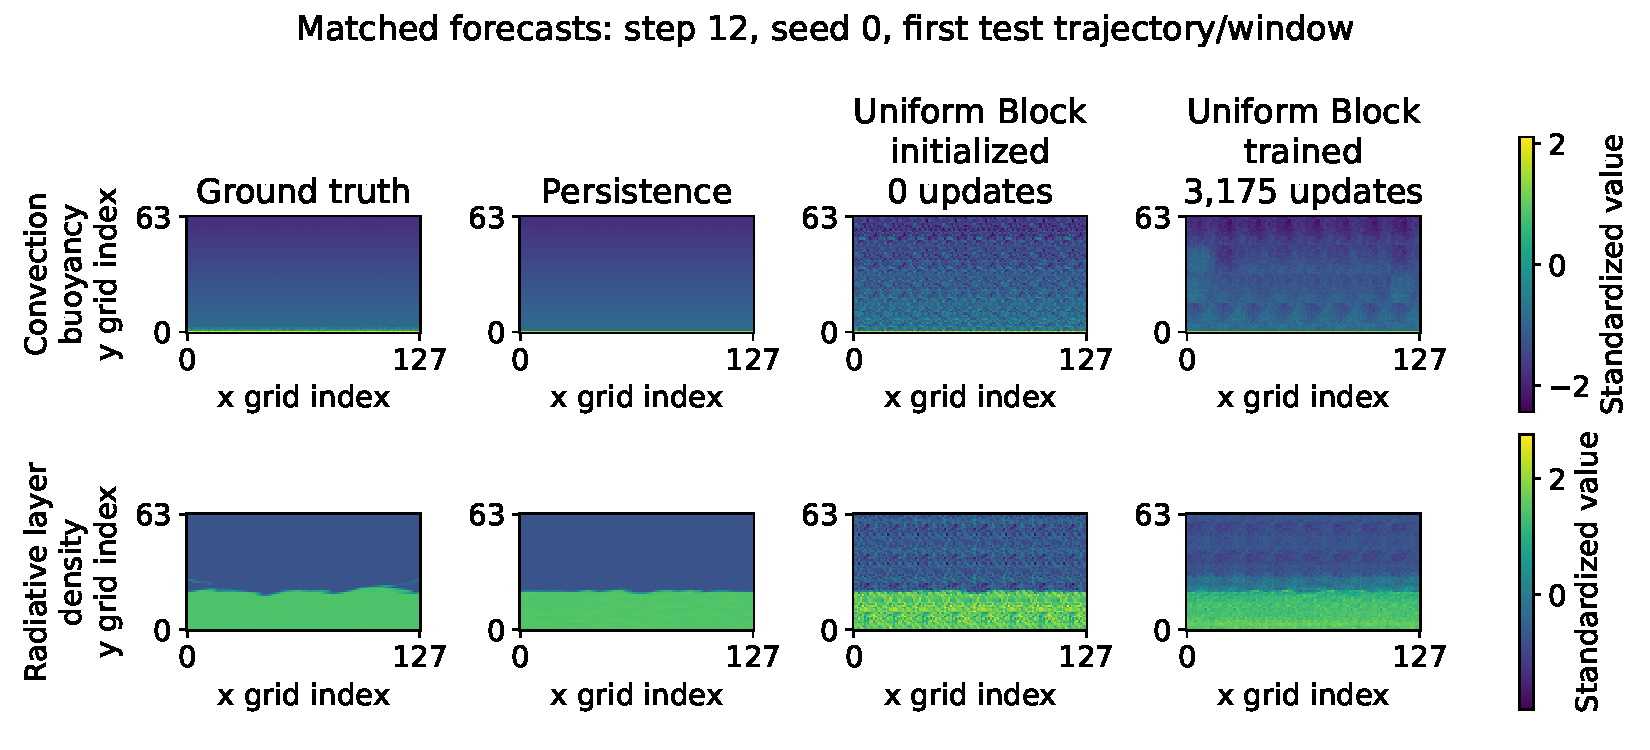
\includegraphics[width=\linewidth]{../reports/figures/initialization_uniform_block.pdf}\caption{Initialized versus trained Uniform Block: ground truth, persistence, zero-update model, and final trained checkpoint. Both rows use the same seed-zero first test trajectory/window at forecast step twelve, with one common unclipped color range per row. Top: convection buoyancy; bottom: radiative density. Magenta denotes nonfinite values. These fixed illustrative cases do not replace evaluation over all trajectories and seeds.}\end{figure}

\FloatBarrier
% Global: interpret evidence within the tested domain; local: no placeholder numerical claims.
\section{Discussion, claims, and implications}
The experiment separates a practical architecture comparison from a mechanistic question. A Standard--Block difference estimates the total effect of replacing residual composition under the matched training protocol. The Uniform Block control helps assess whether learned selection contributes beyond the change to normalized averaging, but its three-seed sample is exploratory. Interventions on trained Block weights examine immediate routing dependence while retaining the learned backbone; they are not interchangeable with training a uniform-routing model from scratch.

Until all primary pairs are evaluated, this manuscript establishes an implementation and a prospective test, not a forecast-quality improvement. A negative or inconclusive result remains informative about this particular low-budget, coarse-grid regime. Neither a positive local result nor a null result establishes behavior at foundation-model scale, unseen physical systems, different data volumes, or other residual block sizes.

\section{Limitations}
Six independent pairs constrain both power and the precision of variance estimates. Three-seed controls cannot support broad systematic claims. The confidence interval is conditional on selected trajectories and its normality approximation; no claim of coverage under arbitrary effect distributions is made. Matching optimizer updates does not match wall-clock compute because routing architectures have different costs. Conversely, equal compute would change the data exposure and is not the primary comparison specified here.

Coarsening removes unresolved spatial structure and changes numerical divergence residuals. Training-standardized NMSE can strongly weight low-energy targets despite the fixed stabilizer. The model learns a mixture of temporal strides without an explicit stride token, preserving the upstream forward interface; this may limit temporal identifiability. A 12-step endpoint is not a guarantee of asymptotic dynamical stability. GPU execution can vary across hardware and library versions even with deterministic algorithms requested\cite{pytorchrepro}. All these limitations apply regardless of the sign of the observed effect.

\section{Conclusion}
The study defines a reproducible test of depth-wise learned residual routing in the released GPhyT architecture, with matched seeds, controlled source scheduling, held-out autoregressive evaluation, and a finite compute budget. The accompanying measured-results section determines which accuracy and stability conclusions, if any, the completed runs support. Execution correctness and prospective power alone do not answer the primary scientific question.

% Global: primary-source bibliography; local: direct source links support reproducibility.
\begin{thebibliography}{99}
\raggedright
\bibitem{gphyt} F. Wiesner, Z. J. Gray, M. Wessling, and S. Baek. \emph{Towards a Physics Foundation Model}. 2025; version 4, 2026. \url{https://arxiv.org/abs/2509.13805}.
\bibitem{gphytcode} F. Wiesner et al. \emph{General Physics Transformer source code}, commit df1527c4773ababc6f8af0d117fb5803fa3bf74b. \url{https://github.com/FloWsnr/General-Physics-Transformer}.
\bibitem{attnres} Kimi Team. \emph{Attention Residuals}. 2026. \url{https://arxiv.org/abs/2603.15031}.
\bibitem{fla} FLA contributors. \emph{Naive Attention Residuals operator}, commit a400aff6ec0eb81cc88721aedba782cd7d535357. \url{https://github.com/fla-org/flash-linear-attention/blob/a400aff6ec0eb81cc88721aedba782cd7d535357/fla/ops/attnres/naive.py}.
\bibitem{well} R. Ohana et al. \emph{The Well: a Large-Scale Collection of Diverse Physics Simulations for Machine Learning}. NeurIPS Datasets and Benchmarks, 2024. \url{https://arxiv.org/abs/2412.00568}.
\bibitem{wellrelease} Polymathic AI. \emph{The Well release notes: uniform Rayleigh--B\'enard correction}. \url{https://github.com/PolymathicAI/the_well/releases/tag/v1.1.0}.
\bibitem{fastattnres} Fast-AttnRes contributors. \emph{Fast-AttnRes}. \url{https://github.com/jon123boss/fast-attnres}.
\bibitem{liger} Liger Kernel contributors. \emph{Attention Residuals operator}. \url{https://github.com/linkedin/Liger-Kernel/blob/main/src/liger_kernel/ops/attn_res.py}.
\bibitem{nktkt} nktkt. \emph{Attention Residuals implementation}. \url{https://github.com/nktkt/attention-residuals}.
\bibitem{lones} M. A. Lones. \emph{How to avoid machine learning pitfalls: a guide for academic researchers}. 2021. \url{https://arxiv.org/abs/2108.02497}.
\bibitem{lipton} Z. C. Lipton and J. Steinhardt. \emph{Troubling Trends in Machine Learning Scholarship}. 2018. \url{https://arxiv.org/abs/1807.03341}.
\bibitem{pytorchrepro} PyTorch contributors. \emph{Reproducibility notes}. \url{https://docs.pytorch.org/docs/stable/notes/randomness.html}.
\bibitem{studycode} L. Burian. \emph{General Physics Attention Residuals Transformer: study implementation and artifacts}. 2026. \url{https://github.com/BurnyCoder/general-physics-attention-residuals-transformer}.
\end{thebibliography}

\appendix
% Global: concise reproducibility appendix; local: operational detail is centralized in README/protocol.
\section{Artifacts and audit trail}
The public repository\cite{studycode} contains the locked Python 3.13 environment, retained upstream licenses, source hashes, tests, study configuration, preregistered protocol, prospective power tables, and phase-based CLI. Large data and checkpoints live in a configured project-owned directory. The model release uses tensor-only safetensors weights; local optimizer-resume files are trusted artifacts and are not loaded from arbitrary third parties.

Reproduction proceeds through preparation, CPU tests, prospective power, budgeted GPU verification, profiling, publication of the frozen update count, training, evaluation, analysis, and reporting. The README is the authoritative command reference. Checkpoints preserve optimizer moments, completed update number, CPU/CUDA RNG states, and the independent data-sampling RNG. The learning-rate schedule is reconstructed from the saved update and frozen horizon. The published manifest preserves official split membership and training-only normalization.

\section{Verification scope}
Tests compare the FLA operator with the stated equations and gradients, test zero-query averaging, causal source counts, final aggregation, embedding inclusion, forward-call reset, and preservation of the upstream standard path. Data checks cover field mapping, split duplication, normalization isolation, and fixed forecast origins. Forecasting is structurally separated from future targets. Checkpoint tests restore optimization and sample state. Budget rejection paths retain failed attempts. The dashboard and final PDF require visual verification in addition to numerical tests.

Additional CPU regressions require bitwise equality when uniform or shuffled interventions leave routing weights unchanged, both with and without BF16 autocast. Nonuniform identity-shuffle probes cover learned routing. Separate output and gradient comparisons protect the ordinary FLA training path. The dated architecture audit records the failing and passing checks; CUDA intervention verification remains pending while the original training worker owns the GPU budget.

\section{Reporting policy}
Every planned experiment retains a report even if omitted or failed. Raw per-trajectory metrics, training logs, runtime costs, configuration hashes, and source versions support derived tables. Post-hoc analyses must be labeled separately from the primary endpoint. No reinforcement-learning reward is defined for this supervised regression study, so no reward curve is reported. Public model cards must state the same data, normalization, compute, and scientific limits as this manuscript.

\section*{AI authorship and human revision statement}
Codex wrote this codebase and paper. A human provided the exact specification that Codex executed. Human cleanup and rewriting are in progress.
\end{document}
